
%%%%%%%%%%%%%%%%%%%%%%%%%%%%%%%%%%%%%%%%
%%%%%%%%%%%%%%          SETUP       %%%%%%%%%%%%%%%%%
%%%%%%%%%%%%%%%%%%%%%%%%%%%%%%%%%%%%%%%%

%%% DOCUMENT CLASS
% NOTE: remove "handout" from the document class and everything will reveal in stepwise fashion, including inserted pauses
\documentclass[12pt, compress, handout]{beamer} 

%%% PACKAGES
\usepackage[english]{babel}
\usepackage{graphicx}
\usepackage[absolute,overlay]{textpos} % to get full size picture
\usepackage{tabulary} % for wrapping tables
\usepackage{csquotes}
\usepackage{hyperref}
\usepackage{fontspec}
\usepackage{etoolbox}

%%% IMAGES
\graphicspath{{images/}} % simplifies directory for graphics path

%%% FRAME TITLES
\setbeamertemplate{frametitle}[default][center] % centering titles
\addtobeamertemplate{frametitle}{\vspace*{.6cm}}{\vspace*{0.2cm}} % title space

%%% NAVIGATION 
\beamerdefaultoverlayspecification{<+->} % uncovers everything step-wise
\beamertemplatenavigationsymbolsempty % gets rid of navigation menu
\makeatletter
\patchcmd{\slideentry}{\advance\beamer@xpos by1\relax}{}{}{}
\def\beamer@subsectionentry#1#2#3#4#5{\advance\beamer@xpos by1\relax}%
\makeatother
\setbeamertemplate{footline} % adds sections and subsection dots in footnote
{
	\begin{beamercolorbox}[center]{section in head/foot}
	\vskip12pt % distance from top 
	\insertnavigation{\paperwidth}
	\vskip4pt % distance from bottom
	\end{beamercolorbox}
}

%%%%% COLORS 
\definecolor{textcolor}{RGB}{24,24,24} % sets main text color
\definecolor{background}{RGB}{255,255,255} % sets background to white
\definecolor{burntorange}{rgb}{0.8, 0.33, 0.0}
\definecolor{ceruleanblue}{rgb}{0.16, 0.32, 0.75}
\definecolor{gray}{RGB}{155,155,155}
\setbeamercolor{titlelike}{fg=ceruleanblue}
\setbeamercolor{subtitle}{fg=burntorange}
\setbeamercolor{framesubtitle}{fg=ceruleanblue}
\setbeamercolor{section title}{fg=burntorange} 
\setbeamercolor{institute}{fg=gray}
\setbeamercolor{normal text}{fg=textcolor, bg=background} 
\setbeamercolor{item}{fg=burntorange}
\setbeamercolor{enumerate}{fg=burntorange}
\hypersetup{colorlinks, linkcolor=, urlcolor=burntorange} 
\let\oldtexttt\texttt% Store \texttt
\renewcommand{\texttt}[2][ceruleanblue]{\textcolor{#1}{\ttfamily #2}}

%%%%% FONTS 
\usefonttheme{professionalfonts}
\usefonttheme{serif}
\setmainfont[Ligatures=TeX]{Helvetica Light} % ligatures for em dash quotes
\setbeamerfont{note page}{family*=pplx, size=\footnotesize} % Palatino for notes
\setbeamerfont{section title}{size=\Huge, series=\bfseries}
\setbeamerfont{subsection title}{size=\huge}
\setbeamerfont{framesubtitle}{size=\small} 
\urlstyle{same} % make URLs in normal font, not mono-spaced

%%%%% SECTION TITLE SLIDES
\AtBeginSection[]{
  \begin{frame}
  \vfill
  \centering
  \begin{beamercolorbox}[center]{title}
  	\vskip14pt
    \usebeamerfont{section title}\usebeamercolor[fg]{section title}\insertsectionhead\par%
  \end{beamercolorbox}
  \vfill
  \end{frame}
}

\AtBeginSubsection[]{
  \begin{frame}
  \vfill
  \centering
  \begin{beamercolorbox}[center]{title}
  	\vskip14pt
    \usebeamerfont{subsection title}\insertsubsectionhead\par %
  \end{beamercolorbox}
  \vfill
  \end{frame}
}

%%%%% SPACING
\let\noteitem\item % increase spacing between items
\renewcommand{\item}{ 
	\noteitem\vspace{\fill}
	}
\setlength{\tabcolsep}{1em} % horizontal padding for tables 

%%%%% COMMANDS
\newcommand{\ig}{\includegraphics}
\newcommand{\nb}[1]{{\color{burntorange} {#1}}}

%%%%%%%%%%%%%%%%%%%%%%%%%%%%%%%%%%%%%%%%
%%%%%%%%%%%%%%         TITLE       %%%%%%%%%%%%%%%%%%
%%%%%%%%%%%%%%%%%%%%%%%%%%%%%%%%%%%%%%%%

%%%%% TITLE MATERIAL %%%%

\title[Short Title]{How to improve the credibility of (your) social science}
\subtitle{A practical guide for researchers \vspace{-20pt} }
\institute{\vspace{10pt} \ig[width = 40mm]{pdel.png}\vspace{10pt} \ig[width = 20mm]{UCSDlogo}}
%\author{} % add presenter here
\date[Short Occasion]{\today} 

%%%%% BEGIN

	\begin{document}

%%%%% TITLE PAGE

{\setbeamertemplate{footline}{} % no navigation
\frame{
  \titlepage
  \note{}
  }
}

%%%%%%%%%%%%%%%%%%%%%%%%%%%%%%%%%%%%%%%%
%%%%%%%%%%%%%%%   PART 1. PROBLEM    %%%%%%%%%%%%%
%%%%%%%%%%%%%%%%%%%%%%%%%%%%%%%%%%%%%%%%

\section{The Problem}
\subsection{}
	\begin{frame}
		\centering
		\ig[width=\textwidth]{jelly1.png}
	\end{frame}

	\begin{frame}
		\centering
		\ig[width=\textwidth]{jelly2.png}
	\end{frame}

	\begin{frame}
		\centering
		\ig[width=\textwidth]{jelly3.png}
	\end{frame}

	\begin{frame}
		\centering
		\ig[width=\textwidth]{jelly4.png}
		
		\href{https://xkcd.com/882/}{Source: XKCD}
	\end{frame}
	
	\begin{frame}{We often hear about ... }
		\begin{enumerate}
			\item \textbf{``Replication crisis"}---studies fail to replicate (psych, econ, polisci, medicine, etc.)
			\item \textbf{Publication bias}---published studies only represent fraction of results, biased toward significant positive findings
			\item \textbf{P-hacking/researcher degrees of freedom}---published studies use only a fraction of possible specifications, biased toward significance 
			\item \textbf{Misconduct/fraud}---relatively easy to get away with!
		\end{enumerate}			
		\bigskip
		
		\pause
		\centering
		$\rightarrow$ adds up to \nb{biased body of knowledge} 
	\end{frame}

	\begin{frame}{Why do we have this credibility crisis?}
		\centering
		\ig[width=.8\textwidth]{problems.png}
	\end{frame}
	
	
%%%%% REPLICATION CRISIS	
	\subsection{1. ``Replication Crisis"}
	
	\begin{frame}{Social, behavioral, and medical \\ studies often don't replicate}		
		\begin{itemize}
			\item \nb{\textbf{Ideally}}, replications determine if original results are robust to alternative specifications or if they were due to \textit{random chance}.
			\item \nb{\textbf{In reality}}, failure to replicate often a result of ...
					\begin{itemize}
						\item Lack of transparency in sharing data/code
						\item Errors in data/code
						\item Misconduct or fraud 
					\end{itemize}
		\end{itemize}
	\end{frame}
		
	\begin{frame}{Dewald et al. (1986)}
	\centering
	Attempted to replicate papers submitted to \textit{Journal of Money, Credit and Banking}:
	
	\centering
	\bigskip
	\ig[width=.9\textwidth]{dewald.png}
		
	\end{frame}
	
	\begin{frame}{Fang et al. (2012)}
		Review of 2,047 retracted biomedical and life-science articles on PubMed:
		
		\centering
		\bigskip
		\ig[width=.7\textwidth]{fang2012.png}
	\end{frame}

%%%%% PUBLICATION BIAS

	\subsection{2. Publication Bias}

	\begin{frame}{AKA the ``file drawer problem"}
		\begin{itemize}
			\item \textbf{Problem:} Studies more likely to be submitted/published when findings are significant $\rightarrow$ studies with null (or negative) findings are hidden
			\item \textbf{Result:} Bias evidence base—we're missing full universe of studies and results; what gets published could be due to random chance (e.g., if we expect 5\% of results of all studies to be significant)
		\end{itemize}		
	\end{frame}

	\begin{frame}{Fanelli (2010 \& 2011)}
		\centering
		Increase in \% of papers with positive results over time, across scientific disciplines:
		
		\bigskip
		\ig[width=\textwidth]{fanelli2011.png}
	\end{frame}
	
	\begin{frame}{Franco, Malhotra, Simonovits (2014)}
		\centering
		Strong results 60pp more likely to be written up than null results, 40pp more likely to be published:
		
		\bigskip
		\ig[width=\textwidth]{franco2014.png}
	\end{frame}

	\begin{frame}{This has consequences!}
		\centering
		E.g., studies that agree with FDA decisions more likely to be published (Turner et al. 2008):
		
		\bigskip
		\centering
		\ig[width=.5\textwidth]{turner2008a.png}	
	\end{frame}
	
%%%%% P-HACKING

	\subsection{3. P-hacking---AKA fishing, data mining, specification searching, etc.}

	\begin{frame}{``Torture the data until it tells you what you want to hear"}
		\begin{itemize}
			\item \textbf{Opportunity:} Researchers also have many \nb{``degrees of freedom" (RDF)} in the design and analysis of a study $\rightarrow$ p-hacking (may not always be intentional, see Gelman \& Loken 2013)
			\item \textbf{Motive:} Researchers have incentives (from journals, tenure requirements, etc.) to find significance
			\item \textbf{Result:} Biased evidence base (also contributes to replication crisis)
		\end{itemize}
	\end{frame}
	
	\begin{frame}{Brodeur et al. (2016)}
		\centering
		Evidence of P-Hacking:
		
		\bigskip
		\ig[width=\textwidth]{brodeur2016.png}
	\end{frame}
	
	\begin{frame}{Wicherts et al. (2016)}
		Identify 34 key researcher DFs (see \href{https://osf.io/umq8d/}{article} for full list):
		
		\bigskip
		\ig[width=\textwidth]{wicherts2016.png}
		...
	\end{frame}

%%%%% MISCONDUCT & FRAUD	

	\subsection{4. Misconduct \& Fraud}

	\begin{frame}{Rare(?) but serious}
		\begin{itemize}
			\item \textbf{Includes}: Falsifying some or all data and/or results, as well as plagiarism and other forms of misconduct
			\item \textbf{Result:} False or biased evidence base,  (also contributes to replication crisis)
			\item \nb{\textbf{Note}:} Fabrication of data (e.g., \href{https://fivethirtyeight.com/features/how-two-grad-students-uncovered-michael-lacour-fraud-and-a-way-to-change-opinions-on-transgender-rights/}{LaCour}, \href{http://nautil.us/issue/24/error/how-the-biggest-fabricator-in-science-got-caught}{Fujii}, \href{http://andrewgelman.com/2014/06/24/linear-true-curious-case-jens-forster/}{Foster}, \href{https://www.theguardian.com/science/2017/feb/01/high-tech-war-on-science}{Staple}) less common than other ``questionable research practices"
		\end{itemize}
	\end{frame}
	
	\begin{frame}{John et al. (2012)}
		 \centering
		 Survey of 2000 psychologists on questionable practices:
		 
		 \ig[width=.9\textwidth]{john2012.png}
	\end{frame}

%%%%% SOLUTIONS	

	\subsection{But all hope is not lost ...}
	
	\begin{frame}{Norms are changing}
		Smart people are working on these issues and developing standards and tools to help throughout the \nb{research lifecycle}. 
	
		\pause		
		\begin{itemize}
				\item PDEL, BITSS, OSF, DART, Dataverse, EGAP, etc. etc. 
			\end{itemize}
		\end{frame}

	\begin{frame}{Research lifecycle: Individual-level solutions}
	\centering
		\ig[width=\textwidth]{lifecycle.png}
	\end{frame}

%%%%%%%%%%%%%%%%%%%%%%%%%%%%%%%%%%%%%%%%
%%%%%%%%%%%%%%%  PART 2. SOLUTIONS  %%%%%%%%%%%%%
%%%%%%%%%%%%%%%%%%%%%%%%%%%%%%%%%%%%%%%%


%%%%%%%%%%%%%  	SOLUTIONS 1: DESIGN	 %%%%%%%%%%%%%%
\section{Solutions I: Design}

	\begin{frame}{Steps}
	  	\centering
	  	\ig[width=\textwidth]{i_design}
	\end{frame}

%%%%% REGISTRATION	

\subsection{1. Registration}

	\begin{frame}{About Registration}
		\begin{itemize}
			\item \textbf{What:} Enter your study into the appropriate disciplinary ``registry"---basically a requirement for experiments (especially in medicine)
			\item \textbf{Why:} To combat the file-drawer problem, publication bias--- also, stake out intellectual claim!
		\end{itemize}
	\end{frame}
	
	\begin{frame}{Where to Register}
		\begin{itemize}
			\item \textbf{American Economics Association (AEA):} \url{http://socialscienceregistry.org}
			\item \textbf{Experiments in Governance and Politics (EGAP):} \url{http://egap.org/design-registration}
			\item \textbf{Registry for International Development Impact Evaluations (3ie):} \url{http://ridie.3ieimpact.org}
			\item \textbf{Open Science Framework:} \url{http://osf.io}---OSF is integrated with other formats, soon with AEA!
			\item \url{http://aspredicted.org}
		\end{itemize}
		\end{frame}
	
	\begin{frame}{AEA}
		To register an experimental study with AEA ...
		
		\pause
		\begin{enumerate}
			\item Create an account at \url{https://www.socialscienceregistry.org}
			\item Click on ``register a trial" and enter basic information---including title, country, status, keyword, abstract, start and end dates, outcomes, experimental design, whether treatment clustered, planned number of clusters and observations, IRB information
		\end{enumerate}
	\end{frame}	
		
	\begin{frame}{EGAP}
		To register an experimental (or non-experimental) study with EGAP ... 
		
		\pause
		\begin{enumerate}
			\item If you're not already in the EGAP author database, go to \url{http://egap.org/node/add/people} to add your name and basic information 
			\item Go to \url{http://egap.org/node/add/registration} and complete the registration form---including faculty affiliation, prospective vs. retrospective, whether experimental, start date, background on study, hypotheses to be tested, basic research design, sample size, whether power analysis, IRB information, and keywords
		\end{enumerate}
	\end{frame}	

%%%%% PRE-ANALYSIS PLANS	
	
\subsection{2. Pre-Analysis Plan}

	\begin{frame}{About Pre-Analysis Plans (PAPs)}
		\begin{itemize}
			\item \textbf{What:} Detailed description of research design and data analysis plans, submitted to a registry BEFORE looking at the data.
			\item \textbf{Why:} 
				\begin{itemize}
				 	\item Tie your hands for data analysis (address researcher degrees of freedom, etc.)
				 	\item Distinguish between \textit{confirmatory} and \textit{exploratory} analysis
				 	\item Boost credibility of research (get a badge from OSF!)
				 	\item Transparent methods make it easier for others to build on your work
				\end{itemize}
		\end{itemize}
	\end{frame}
	
	\begin{frame}{PAP vs. Registration}
		Registration often---but not always---includes a pre-analysis plan. BUT, purpose is different ...
		
		\pause	
		\begin{itemize}
			\item \textbf{Registration addresses publication bias}---study enters the universe, no matter the outcome 
			\item \textbf{PAP addresses p-hacking}---limiting degrees of freedom
		\end{itemize}	
		\bigskip
	\end{frame}

	\begin{frame}{Where to Submit a PAP}
		Generally, upload as \textit{part} of registration process ...
		
		\pause
		\begin{itemize}
			\item \textbf{American Economics Association (AEA):} \url{http://socialscienceregistry.org} 
			\item \textbf{Experiments in Governance and Politics (EGAP):} \url{http://egap.org/design-registration}
			\item \textbf{Registry for International Development Impact Evaluations (3ie):} \url{http://ridie.3ieimpact.org}
			\item \textbf{Open Science Framework:} \url{http://osf.io}
		\end{itemize}
	\end{frame}	
		
	\begin{frame}{\textbf{OSF}}
		\begin{itemize}
			\item Goal is one-stop hub for transparency across scientific disciplines
			\item Make an account and explore at \url{https://osf.io/}
			\item Win \$1000 with \href{https://osf.io/prereg/}{Preregistration Challenge}
		\end{itemize}
	\end{frame}
	
	\begin{frame}{No universal standard, can include ... }
		\footnotesize
		\begin{table}[H]
		  \begin{tabulary}{\textwidth}{l L}
		    \nb{Background} & abstract, motivation, questions \\[5pt]
		    \nb{Design} & treatment, sampling \& randomization, attrition, spillover, survey instruments, power calculations, plan for data collection, processing \& management \\[5pt]
		    \nb{Analysis} & hypotheses (main, auxiliary), outcome measures (primary, secondary), variable operationalization, balance checks, estimation of treatment effects (ATE, ITT, TOT, etc.), HTEs (subgroups, interactions), covariates, standard errors, corrections for multiple hypothesis testing, missing values, outliers \\[5pt]
		    \nb{Team} & members, affiliations, conflicts of interest \\[5pt]
		    \nb{Logistics} & fieldwork, timeline, budget \\
		  \end{tabulary}
		\end{table}
	\end{frame}
	
	\begin{frame}{Olken's PAP Checklist (2013)}
		\ig[width = \textwidth]{olken2013.png}
	\end{frame}
	
	\begin{frame}{Tie your hands in the right places}
			\centering
			\ig[width = .8\textwidth]{pap_scale.png}
			
			\pause
			\bigskip
			 $\rightarrow$ \textbf{requires a lot of thought!} 
	\end{frame}

	\begin{frame}{Ongoing Debate}
		\begin{itemize}
			\item \href{https://www.aeaweb.org/articles?id=10.1257/jep.29.3.61}{Olken (2013)} on ``Promises and Perils of Pre-analysis Plans"
			\item \href{https://www.aeaweb.org/articles?id=10.1257/jep.29.3.81}{Coffman \& Niederle (2015)} argue that ``Pre-analysis Plans Have Limited Upside, Especially Where Replications Are Feasible"
			\item More debate on utility for observational work but can be done (see \href{http://onlinelibrary.wiley.com/doi/10.1111/0019-8676.00199/full}{Neumark 2001})
		\end{itemize}
	\end{frame}

%%%%% IRB

\subsection{[IRB]}

	\begin{frame}{Not covered here, but ...}
		Don't forget \nb{IRB requirements} to protect human subjects! 
		
		\pause
		\bigskip
		Necessary for ethical research, though not sufficient (see \url{http://desposato.org/ethicsfieldexperiments.pdf} for more on ethics in experiments).
	\end{frame}

%%%%%%%%%%%%%  	SOLUTIONS 2: ANALYSIS %%%%%%%%%%%%

\section{Solutions II: Analysis}

	\begin{frame}{Steps}
	\centering
		``\textbf{Reproducibility} is just collaboration with people you don’t know, including yourself next week" --- Philip Stark, UC Berkeley
		
		\bigskip
			\ig[width=\textwidth]{ii_analysis.png}
	\end{frame}
	
%%%%% FILE MANAGEMENT

\subsection{3. File Management}	

	\begin{frame}{About File Management}
		\begin{itemize}
			\item \textbf{What:} Organizing and managing files cleanly and intuitively
			\item \textbf{Why:} To preserve original data, streamline workflow, and reduce prep time when sharing files
		\end{itemize}
	\end{frame}

	\begin{frame}{Don't let your files look like this ... }
		\centering
		  \ig[width= .80\textwidth]{bad_file_structure}
	\end{frame}	
	
	\begin{frame}{Instead, use PDEL template (or similar)}
	\centering
	Download at \url{https://github.com/PolicyDesignEvaluationLab/Transparency-Initiative}
			\begin{figure}[H]
			  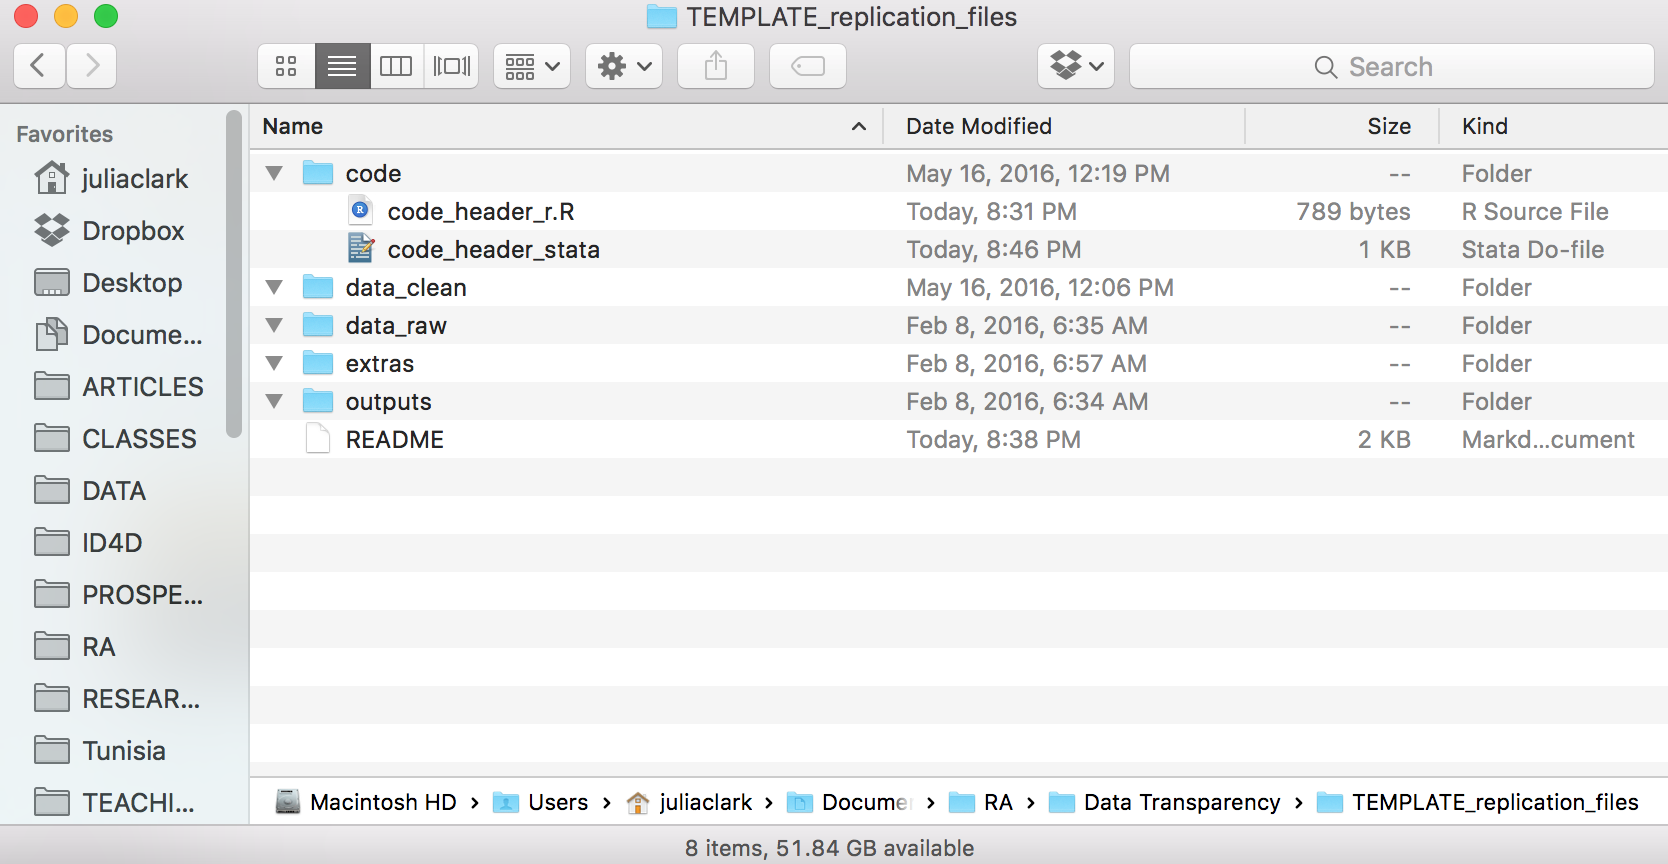
\includegraphics[width= \textwidth]{pdel_structure}
			\end{figure}
	\end{frame}
	
%%%%% LITERATE PROGRAMMING	
	
\subsection{4. Literate Programming}	

	\begin{frame}{About Literate Programming}
		\begin{itemize}
			\item \textbf{What:} Writing code that it's legible to \textit{humans}
			\item \textbf{Why:} So you and others can better replicate your work (and to help you avoid mistakes!)
		\end{itemize}
	\end{frame}
	
	\begin{frame}{(The Most) Basic Principles}
		\begin{itemize}
			\item Structure and name files intuitively
			\item Make the contents of files easy to navigate
			\item Streamline code to avoid repetition
		\end{itemize}
	\end{frame}
	
	\begin{frame}{Structure and Name Files}
 		
 		\begin{itemize}
 			\item	 Create separate scripts for merging/cleaning and data analysis, with a master-script for running it all
 			\item Give code, data files, and output logical names where possible 
 			\begin{itemize}
 				\item Number scripts sequentially in the order they should be run (e.g., \texttt{1\_main\_analysis.R}, \texttt{2\_robust\_checks.R})
 				\item Label output figures with descriptive names, but ones that aren't likely to change (e.g., \texttt{figure\_hte.png} is better than \texttt{figure\_1.png})
 			\end{itemize}
 		\end{itemize}
 	\end{frame}
 
	 \begin{frame}{Improve navigation}
	 	
	 	\begin{itemize}
	 		\item Add headers (see PDEL template)
	 		\item Format scripts so they're easily readable---e.g., indent code, use ample line breaks and spaces, standardize comment syntax
	 		\item Add comments to improve reader understanding
			\item Clearly label code sections, main analyses, outputs 
			\item Give functions, objects, and variables intuitive names like \texttt{edu\_percent} rather than \texttt{v76}
			\item Label variables and values in Stata
			\end{itemize}
	 \end{frame}
	 	 
	 \begin{frame}{Streamline Code—e.g., working directories}  
			\textbf{R}: \texttt{setwd("$\sim$/Documents/replication\_files")} \\
		 	\textbf{Stata}: \texttt{capture cd "$\sim$/Documents/replication\_files"}
		 	
		 	\bigskip
		 	\pause
			 \begin{itemize}
			 	\item Saves you time, since you (or someone replicating your study) only have to change the path once if the files move AND your code will be shorter
			 	\item Particularly helpful if co-authors alternate between Mac (``/") and Windows (``$\backslash$") file extensions
			 \end{itemize}
	 \end{frame}

	
%%%%% VERSION CONTROL	
	
\subsection{5. Version Control}

	\begin{frame}
	\centering
		\ig[width=.6\textwidth]{phd101212s.png}
	\end{frame}
	
	\begin{frame}{About Version Control}
		\begin{itemize}
			\item \textbf{What:} A system for managing iterative versions of files (code, data, manuscripts) over time and across collaborators
			\item \textbf{Why:} Keep original files, protect work, collaborate efficiently, streamline workflow, etc., etc.
		\end{itemize}
	\end{frame}
	
	\begin{frame}{Principles of Version Control}
		\begin{itemize}
			\item Vault original, raw data files---do not save over!
			\item Changes to files should be documented and reversible
			\item Keep ``master" versions of files in working order; create copies before experimenting
			\item Reconcile independent changes  by different users
		\end{itemize}
	\end{frame}

	\begin{frame}{Manual Solutions (not ideal, but better than nothing)}
			\begin{itemize}
				\item Create dated versions of files (save-as) for each substantive change 
				\item With each modification, re-run ALL code to make sure nothing is broken---helps if you have a master file to run all scripts!
				\item Check-in with coauthors to ensure multiple people aren't working on the same files at the same time
				\item Keep a simple log to remind yourself of the location/content of major changes
			\end{itemize}	
				
	\end{frame}
	
	\begin{frame}{Or let version control software do this for you!}
		\centering 
		\ig[width=\textwidth]{github-logo}
	\end{frame}

%% GITHUB	

	\begin{frame}{Version control software > Git > GitHub}
	
		\begin{itemize}
			\item \textbf{Version control software:} helps manage versions and edits to files (e.g., Microsoft Word's ``track changes", or Google Doc's ``suggestion" feature)---\href{https://en.wikipedia.org/wiki/List_of_version_control_software}{many options!}
			\item \textbf{Git:} Open-source, ``distributed model" of version control developed by creator of Linux
			\item \textbf{GitHub:} Free, web-based service that hosts Git ``repositories" and offers a variety of features for collaboration
		\end{itemize}
	\end{frame}
		
	\begin{frame}{Common problems that GitHub helps solve}
	
		\begin{itemize}
			\item \textbf{Tracking changes in code/text files}---who, what, where, when, preserved forever
			\item \textbf{Selectively reverting changes}---better than \texttt{ctrl + Z}
			\item \textbf{Experimenting}---easier than ``my\_code\_v2\_new.R"
			\item \textbf{Collaborating}---sharing/vetting/reconciling changes
		\end{itemize}
	\end{frame}
		
	\begin{frame}{How do I use GitHub?}
	
		\begin{itemize}
			\item \textbf{GitHub website}---necessary for collaboration, but limitations
			\item \textbf{GitHub Desktop}---free desktop client for Windows/Mac, more user friendly than website
			\item \textbf{Command line (shell)}---optimal for advanced users
		\end{itemize}
	\end{frame}

	\begin{frame}{How to think about Git}
	
		\begin{columns}
			\begin{column}	{.5\textwidth}
				\centering
				\ig[width=.7\textwidth]{Big-brother-poster1.png}
			\end{column}
			\begin{column}{.5\textwidth}
				Tell Git to \nb{watch a set of files} (``repository") and it tracks every change within them, line-by-line.*
				\bigskip
				
				\footnotesize
				\pause
				*If they are text/code files (e.g., .txt, \LaTeX, Markdown, Stata, .R, etc.). Git's not really useful for PDF, Word, Excel (sorry). 
			\end{column}
		\end{columns}
	\end{frame}
	
	\begin{frame}{GitHub is NOT ... }
		\footnotesize
		\begin{columns}
			\begin{column}	{.4\textwidth}
				\centering
				\ig[width=.5\textwidth]{dropbox.png}
				\bigskip
				
				(GitHub.com looks like cloud-based drive, but primary purpose is collaboration, not storage)
			\end{column}
			\begin{column}{.5\textwidth}
				\centering
				\ig[width=.5\textwidth]{finder.png}
				
				\bigskip
				(Desktop app looks like file manager, but use to view changes, not to navigate to/open files)
				\end{column}
			\end{columns}
	\end{frame}

	\begin{frame}{(The most) basic vocabulary}
	
		\begin{itemize}
			\item \nb{\textbf{Repository:}} A set of files (in a folder) that you have told Git to track, along with its associated .git files. \nb{Local} repository = copy on your computer; \nb{remote} repository = copy synced online.
			\item \nb{\textbf{Commit:}} A labeled change or series of changes to files. Git tracks every change you make, and then you group these changes as desired into a ``commit" that can be commented on, reverted, etc.
		\end{itemize}
	\end{frame}
	
	\begin{frame}{10 Baby Steps in Git—Prep}		
		\begin{itemize}
			\item \textbf{Make sure you have a good text editor.} Notepad or TextEdit will work (if you set TextEdit to \texttt{.txt} and not \texttt{.rtf}). Or get a more powerful editor like \href{https://atom.io/}{Atom}. 
			\item \textbf{Create an account at \href{http://www.github.com}{GitHub}.} This gives free \textit{public} repositories, but click ``request a discount" at \href{https://education.github.com/}{} for free \textit{private} repositories. 
			\item \textbf{Download and install \href{https://desktop.github.com/}{GitHub Desktop}.} Then open and log in using your GitHub account.
		\end{itemize}
	\end{frame}

	\begin{frame}{1. Create a NEW repository}
	
	Within \textbf{GitHub Desktop}, click on ``$+$" and then ``create" to make a new repository with a name and location of your choice. This creates a new folder that will be empty except for some hidden files (e.g., a .git directory).
	
		\bigskip \centering
		\ig[width=.8\textwidth]{add_repository.png}
	\end{frame}
		
	\begin{frame}{2. Add a text file to your repository}
	Leave the Desktop app and go to your text editor: 
	
	\pause
		\begin{itemize}
			\item Create a new text file called ``README" and \textit{save it in your repository location}.
			\item  This should be a plain text file (.txt) or Markdown file (.md), NOT a rich text format file (.rtf). 
		\end{itemize}	
	\end{frame}
	
	\begin{frame}{3. Commit this change in GitHub Desktop}
		Commit (i.e., record) your change of adding README by writing a summary and clicking "Commit to master".
		
		\bigskip
		\centering
		\ig[width=.8\textwidth]{add_readme.png}
	\end{frame}

	\begin{frame}{4. Add text to README and commit changes}
		\textbf{Add some text to your file and save.} If you go back to the Desktop client, you will now see something like this: 
		
		\bigskip
		\centering
		\ig[width=.7\textwidth]{edit_readme.png}		
	\end{frame}
	
	\begin{frame}{5. Edit README text and commit changes}
		\textbf{Make and save changes to your text}, then go back to GitHub Desktop. In the right-hand pane, additions will appear in \textcolor{green}{green} and deletions will appear in \textcolor{red}{red}:
			\centering
			\ig[width=.7\textwidth]{edit_readme2.png}
		
		\pause
		\bigskip
		Note that the unit of change is the \textit{paragraph}, so changing ``?" to ``!" involved deleting/adding the whole phrase.
	\end{frame}

	\begin{frame}{6. Undo the last commit}
		If you're unhappy with your LAST commit (i.e., you disliked how it was grouped or labeled), \textbf{click ``Undo"} at the bottom of the screen:
		
		\centering
		\ig[width=.5\textwidth]{undo.png}	
		\pause	
		
		Now, these changes will appear again as "uncommitted changes" for you to regroup or relabel.
	\end{frame}

	\begin{frame}{7. Revert a previous commit}
		If you're unhappy with the CHANGES in a commit themselves, you can \textbf{``revert"} them.$\rightarrow$ \textbf{switch to the ``History" tab} at the and view all your previous commits. Select one, navigate to the dropdown menu, and click \textbf{``Revert"}: 
		
		\bigskip
		\centering
		\ig[width=.8\textwidth]{revert.png}		
	\end{frame}
	
	\begin{frame}{8. Publish repository to your online account}
		We've been working in a \textbf{local repository}--one that that you created on your computer. 
		
		\bigskip
		To collaborate you'll need to publish the repository to the web (i.e., make a \textbf{remote repository}). $\rightarrow$  \nb{\textbf{Click ``publish''}:}
		
			\bigskip
			\centering
			\ig[width=.2\textwidth]{publish.png}	
		
	\end{frame}

	\begin{frame}{9. View your repository \& changes online}
		When you login to GitHub online, you'll see the new repository and file you've added.
			\bigskip
			\centering
			\ig[width=.8\textwidth]{git_online.png}
	\end{frame}
	
	\begin{frame}{10. Edit the file online \& sync with local repository}
		Click on the README file and then click the edit button (the pen). \nb{(A)} \textbf{Make some changes and then commit}. Then go back to the Desktop client and \textbf{click ``Sync"}. \nb{(B)} Your new commit will appear in the \textbf{history tab}.
		
		\bigskip
		\begin{columns}
			\begin{column}	{.5\textwidth}
				\centering
				\nb{(A)}
				\ig[width=\textwidth]{online_edit.png}
			\end{column}
			
			\begin{column}{.5\textwidth}
				\centering
				\nb{(B)}
				\ig[width=\textwidth]{sync.png}
			\end{column}
		\end{columns}

	\end{frame}
	
	\begin{frame}{What's next?}
		That was very very basic. To really use Git, explore these great features with weird names ... 
		
		\pause
		\small
		\begin{itemize}
			\item \textbf{\nb{Forking} online repositories}---duplicates \textit{someone else's} shared repository so you can use/change/build on it without affecting their original work
			\item \textbf{\nb{Cloning} online repositories}---copies an online repository onto your local hard drive
			\item \textbf{\nb{Branching} a repository}---lets you (and others) experiment with changes that can later be merged into the ``master" version
			\item \textbf{Initiating a \nb{pull request}}---submits your commits to be merged into a forked/branched repository (accepted/rejected by collaborators)
		\end{itemize}
	\end{frame}

	\begin{frame}{Git Resources}
	Too many to name, but some good places to start:
	\begin{itemize}
		\item \href{http://www.chronicle.com/blogs/profhacker/a-gentle-introduction-to-version-control/23064}{Gentle intro to version control}
		\item \href{https://www.hastac.org/blogs/harrisonm/2013/10/12/github-academia-and-collaborative-writing}{GitHub and collaborative writing in academia}
		\item \href{http://www.chronicle.com/blogs/profhacker/forks-and-pull-requests-in-github/47753}{Forks and pull requests}
		\item \href{http://blog.scottlowe.org/2015/01/14/non-programmer-git-intro/}{Non-programmer's intro to Git using command line}
		\item \href{http://blog.scottlowe.org/2015/01/27/using-fork-branch-git-workflow/}{Fork-branch workflow using command line (but useful to read for Desktop as well)}
	\end{itemize}
	\end{frame}

%%%%% DYNAMIC DOCS	

\subsection{[Dynamic Docs]}
	\begin{frame}{Not covered here, but ... }
	You can take reproducible research a step further by integrating code \textit{into your manuscript}. 
	
	\pause
	\begin{itemize}
		\item \href{http://rmarkdown.rstudio.com/}{RMarkdown}
		\item \href{http://www.haghish.com/statistics/stata-blog/reproducible-research/markdoc.php}{Stata Markdoc} or \href{http://repec.sowi.unibe.ch/stata/texdoc/}{Stata texdoc}
	\end{itemize}
		
	\end{frame}

%%%%%%%%%%%%  SOLUTIONS 3: DISSEMINATION  %%%%%%%%%
\section{Solutions III: Dissemination}

	\begin{frame}{Steps}
	  	\centering
	  	\ig[width=\textwidth]{iii_dissemination}
	\end{frame}
	
%%%%% PREP FOR REPLICATION	
	
\subsection{6. Prepare for Replication}

	\begin{frame}{Why do we care if our code is reproducible?}
		\begin{itemize}
			\item \textbf{Unselfish reasons}---part of the scientific process and a public good
			\item \textbf{Selfish reasons}---make code more usable for yourself, catch potentially embarrassing errors before they become public, boost your transparency credibility
		\end{itemize}
		
	\end{frame}

	\begin{frame}{Replication files should ...}
	
		\begin{itemize}
			\item Be complete but parsimonious
			\item Run and reproduce results with one click
			\item Be readable and interpretable by humans
			\item Protect personal information
		\end{itemize}
		
		\bigskip
		\pause
		\textbf{Caveat:} There is no single, perfect way to organize or prepare files for replication. Do what works for you (as long as it meets the above criteria)!
	\end{frame}

	\begin{frame}{5 Steps for Prepping Files}
			\begin{enumerate}
				\item Set-up
				\item Initial replication
				\item De-identify
				\item Edit
				\item Final replication
			\end{enumerate}
	\end{frame}
	  
		 \begin{frame}{1. Set Up}
		 	Create a \textit{new}, clearly organized folder structure for replication that you add to selectively.
		 	
		 	\pause
		 	\begin{itemize}
		 		\item \textbf{Purpose:} 
		 		\begin{itemize}
		 			\item Ensure files are \textcolor{burntorange}{complete/parsimonious, legible}
		 			\item Protect original files
		 		\end{itemize}
		 	\end{itemize}
		 	
		 \end{frame}
		  
		 \begin{frame}{Create}
		 	\begin{enumerate}
		 		\item \textbf{A new, empty replication folder} \textit{within} your project directory (e.g., ``\texttt{replication\_files/}") 
		 		\item \textbf{Subfolders:} \textit{Same as File Management tips!}
		 			\begin{itemize}
		 				\item \texttt{code/} --- scripts
		 				\item \texttt{data\_clean/} --- manipulated data
		 				\item \texttt{data\_raw/} --- original data
		 				\item \texttt{output/} --- generated tables, graphs, etc.
		 				\item \texttt{extra/} --- misc. extras (e.g., code book)
		 			\end{itemize}
		 			\item \textbf{A ``README.txt" file} to document contents, sources, software/system versions, other info necessary for replication/comprehension.
		 	\end{enumerate}
		 \end{frame}
		
		 \begin{frame}{2. Initial Replication}
		 	\textit{Copy} (don't move!) data and code files into the replication folder and \nb{try to replicate your results}.
		 	
		 	\bigskip
		 	\pause
		 	\textbf{Purpose:}
			 	\begin{itemize}
			 		\item Make sure your code actually runs and \textcolor{burntorange}{reproduces} before you tinker with structure and formatting
			 		\item Build up your replication folder with \textcolor{burntorange}{complete and parsimonious} data/code files
			 	\end{itemize}
		 \end{frame}
		 
		\begin{frame}{A. Check Analysis}
			Easier to start with final analysis and work backwards to data cleaning/merging. 
			
			\pause
			\begin{enumerate}
				\item Copy original analysis script(s) into \texttt{replication\_files/code}
				\item Copy cleaned dataset(s) used for analysis into \texttt{replication\_files/data\_clean}
				\item Run code without changes (except for wd)
				\item Fix any bugs in the code, address discrepancies with previous results
			\end{enumerate}
		\end{frame}
		
		\begin{frame}{B. Check Data Clean/Merge}
			\begin{enumerate}
				\item If separate from analysis, copy original merge/cleaning script(s) into \texttt{replication\_files/code}
				\item Copy original dataset(s) to \texttt{replication\_files/data}
				\item Run merge/clean code without changes (except for wd)
				\item Rerun the analysis code from above on the newly cleaned/merged data file
				\item If you get different results than step \#1, there is a discrepancy with  merging/cleaning code---fix it!
			\end{enumerate}
		\end{frame}
		
	\begin{frame}{3. De-Identifying Individual-Level Data}
		If you haven't already, make sure replication files \textit{do not contain} data that could be used to identify individuals. 
		
		\bigskip
		\pause
		\textbf{Purpose:} 
		\begin{itemize}
			\item \textcolor{burntorange}{Protect individuals' identity and private information}---ethical issue for researchers, potential safety issue for participants
			\item Comply with legal, research board or funder requirements (e.g., HIPAA and IRB in the US) 
		\end{itemize}
		
	\end{frame}

	\begin{frame}{What does ``de-identifying" mean?}
		\textbf{Two types of identifiers:}
		\pause
		\begin{enumerate}
			\item \textcolor{burntorange}{Direct:} Variables explicitly linked to subjects---\textit{e.g., name, email, address, ID number, phone number, etc.}
			\item \textcolor{burntorange}{Indirect:} Variables that, in combination, could be used to identify individuals---\textit{e.g., gender, dates (birth, program admission, etc.), geographic location (village, GPS), unusual occupations or education, etc.}
		\end{enumerate}
		
		\bigskip
		\pause
		See \href{https://fpf.org/wp-content/uploads/2016/04/FPF_Visual-Guide-to-Practical-Data-DeID.pdf}{this useful infographic}.
	\end{frame}

	\begin{frame}{Example of Indirect Identifiers}	
		\begin{itemize}
			\item You survey teachers and collect information on \textit{gender}, \textit{grade-level taught}, and \textit{age}.
			\item If there is only one \textit{female}, \textit{third-grade} teacher \textit{aged 40-49} at a particular school, she is not anonymous in your data
		\end{itemize}
	\end{frame}		

	\begin{frame}{The Problem}
		 \centering 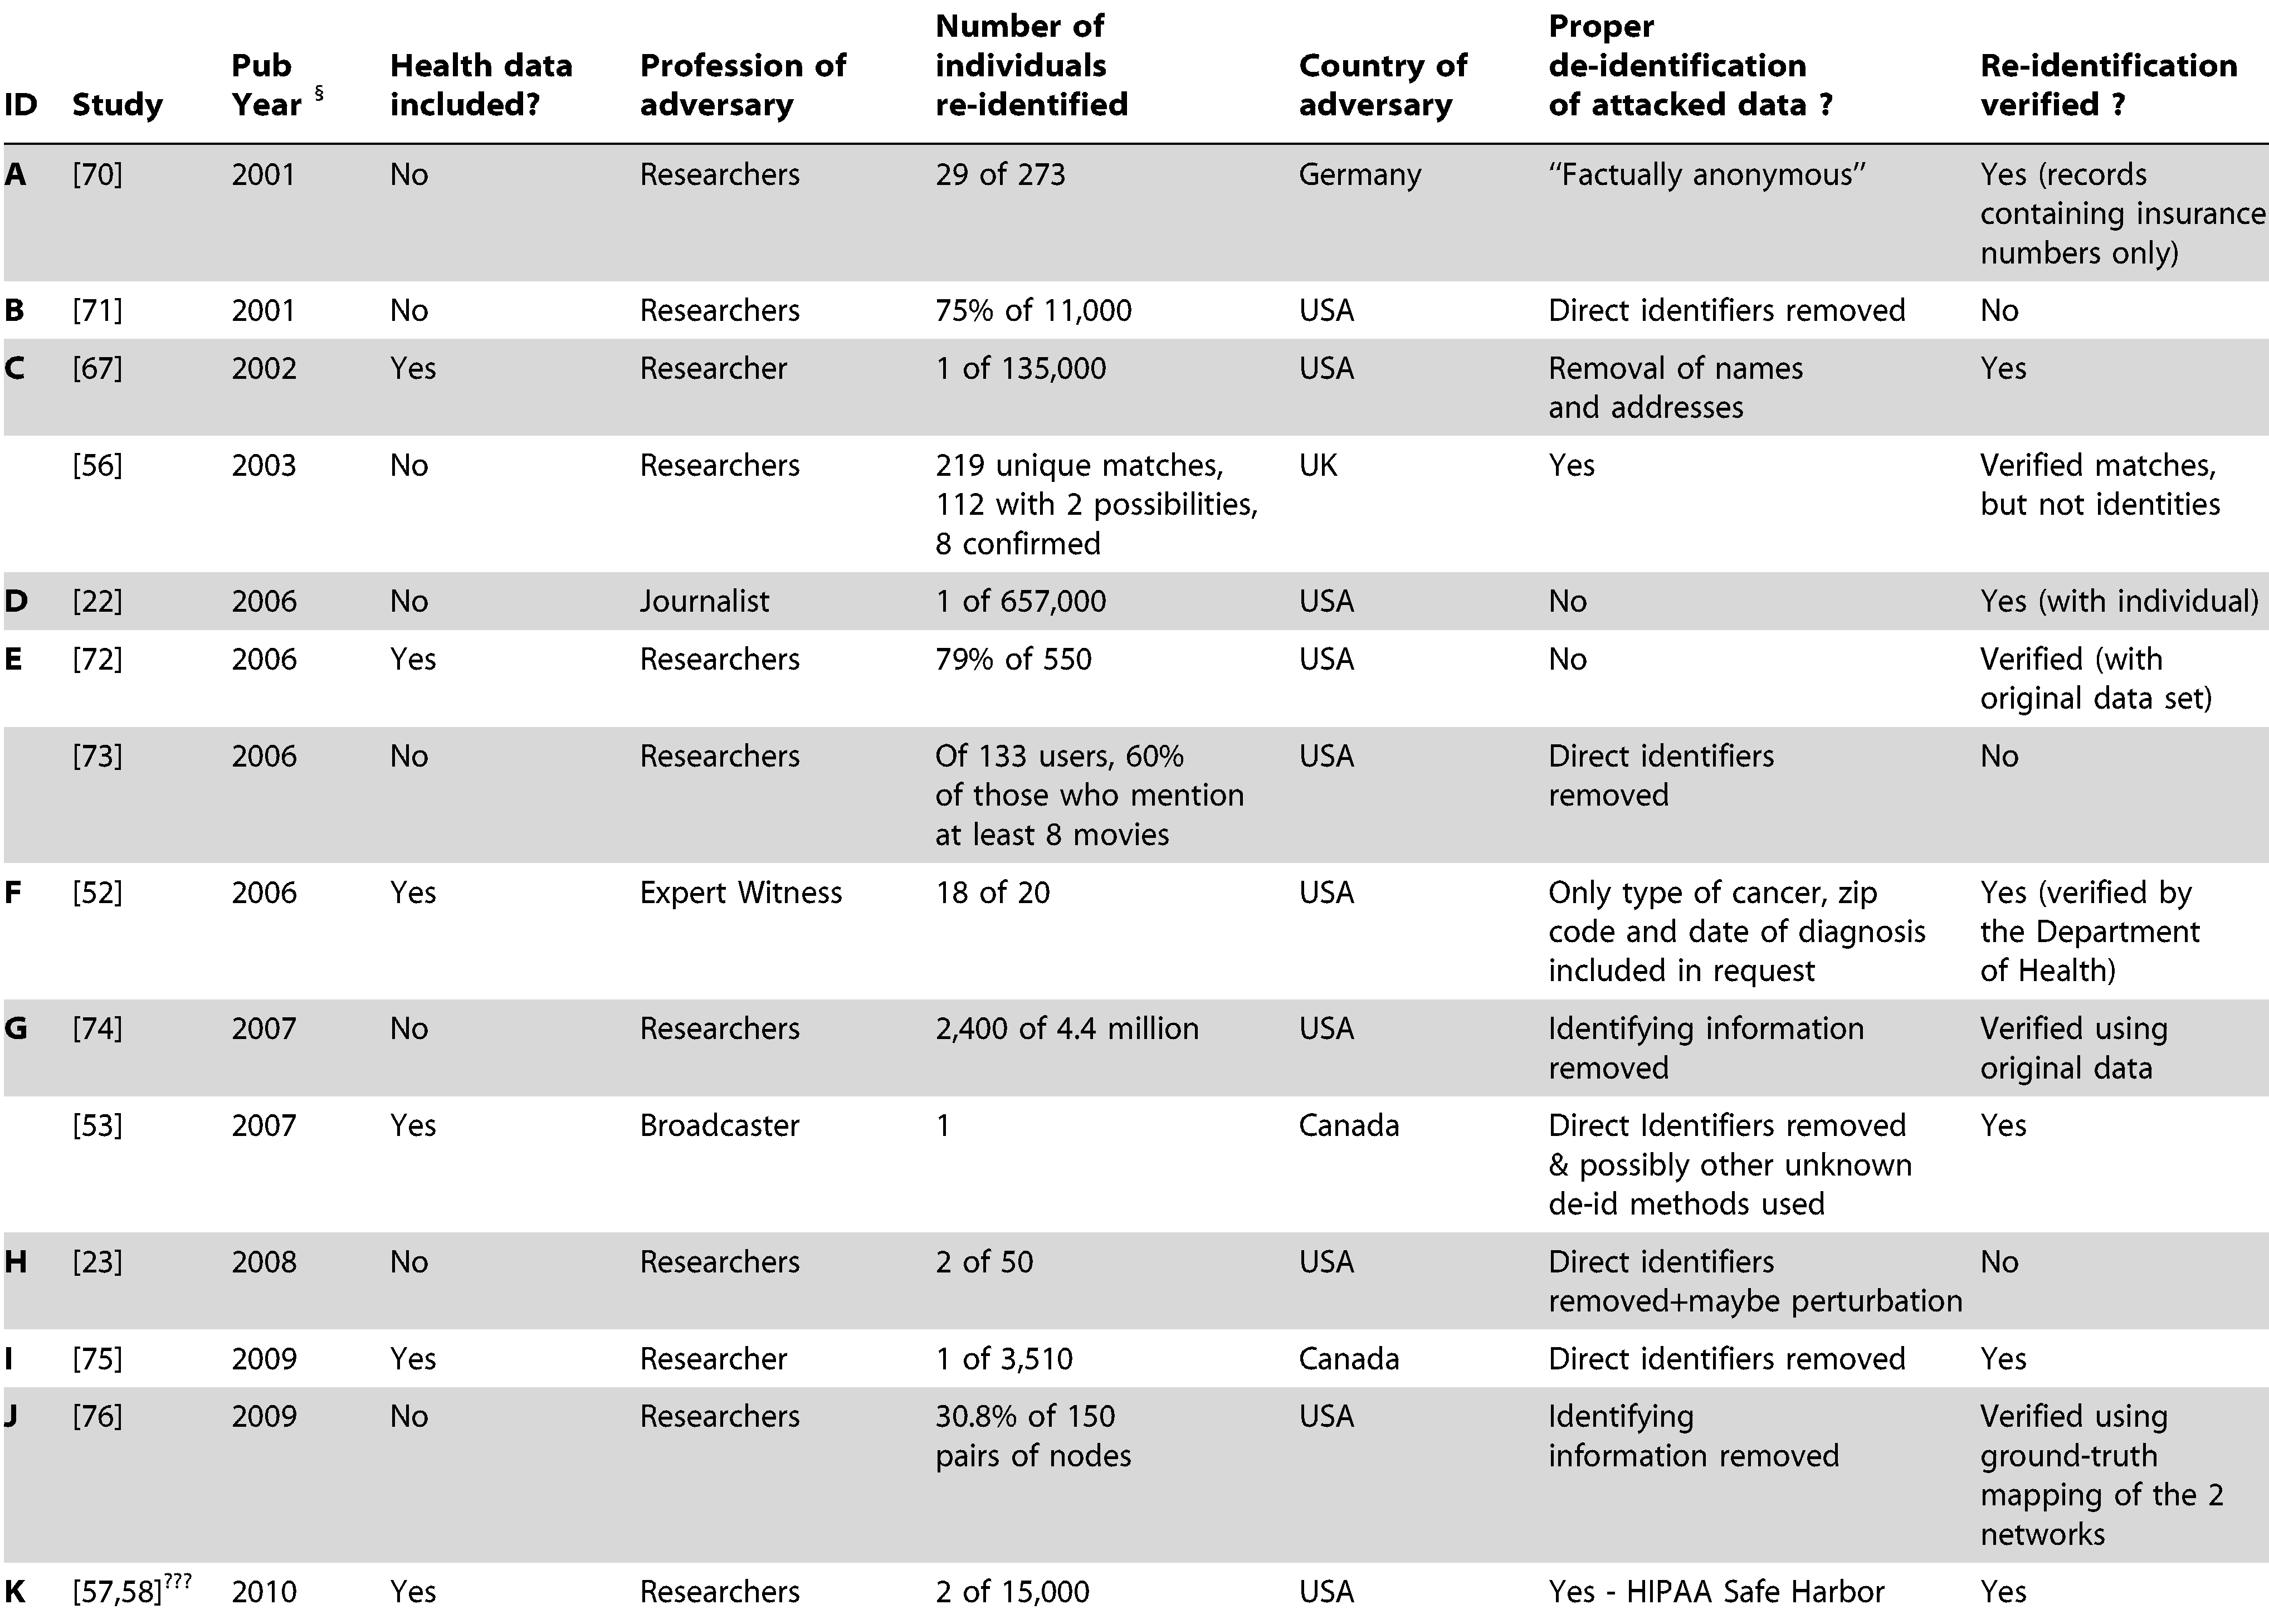
\includegraphics[width=.85\textwidth]{reidentification.png}
		 
		 \tiny{Source: El Emam et al. 2015. ``A Systematic Review of Re-Identification Attacks on Health Data." PLOS One. }
	\end{frame}
	
	\begin{frame}{Dealing with Direct Identifiers}
		In general, direct identifiers---e.g., name, address, mobile number, ID number---should \textit{never} be made public. 
		
		\bigskip
		\pause	
		\textbf{Options:}
		\begin{itemize}
			\item Remove variables from shared dataset
			\item Pseudonymize data in order to be able to link datasets: replace identifiers with ``pseudonyms" that may be reversible or non-reversible, e.g., give people random names or ID numbers
		\end{itemize}
	\end{frame}	
	
	\begin{frame}{Solutions for Direct Identifiers}
		 \centering 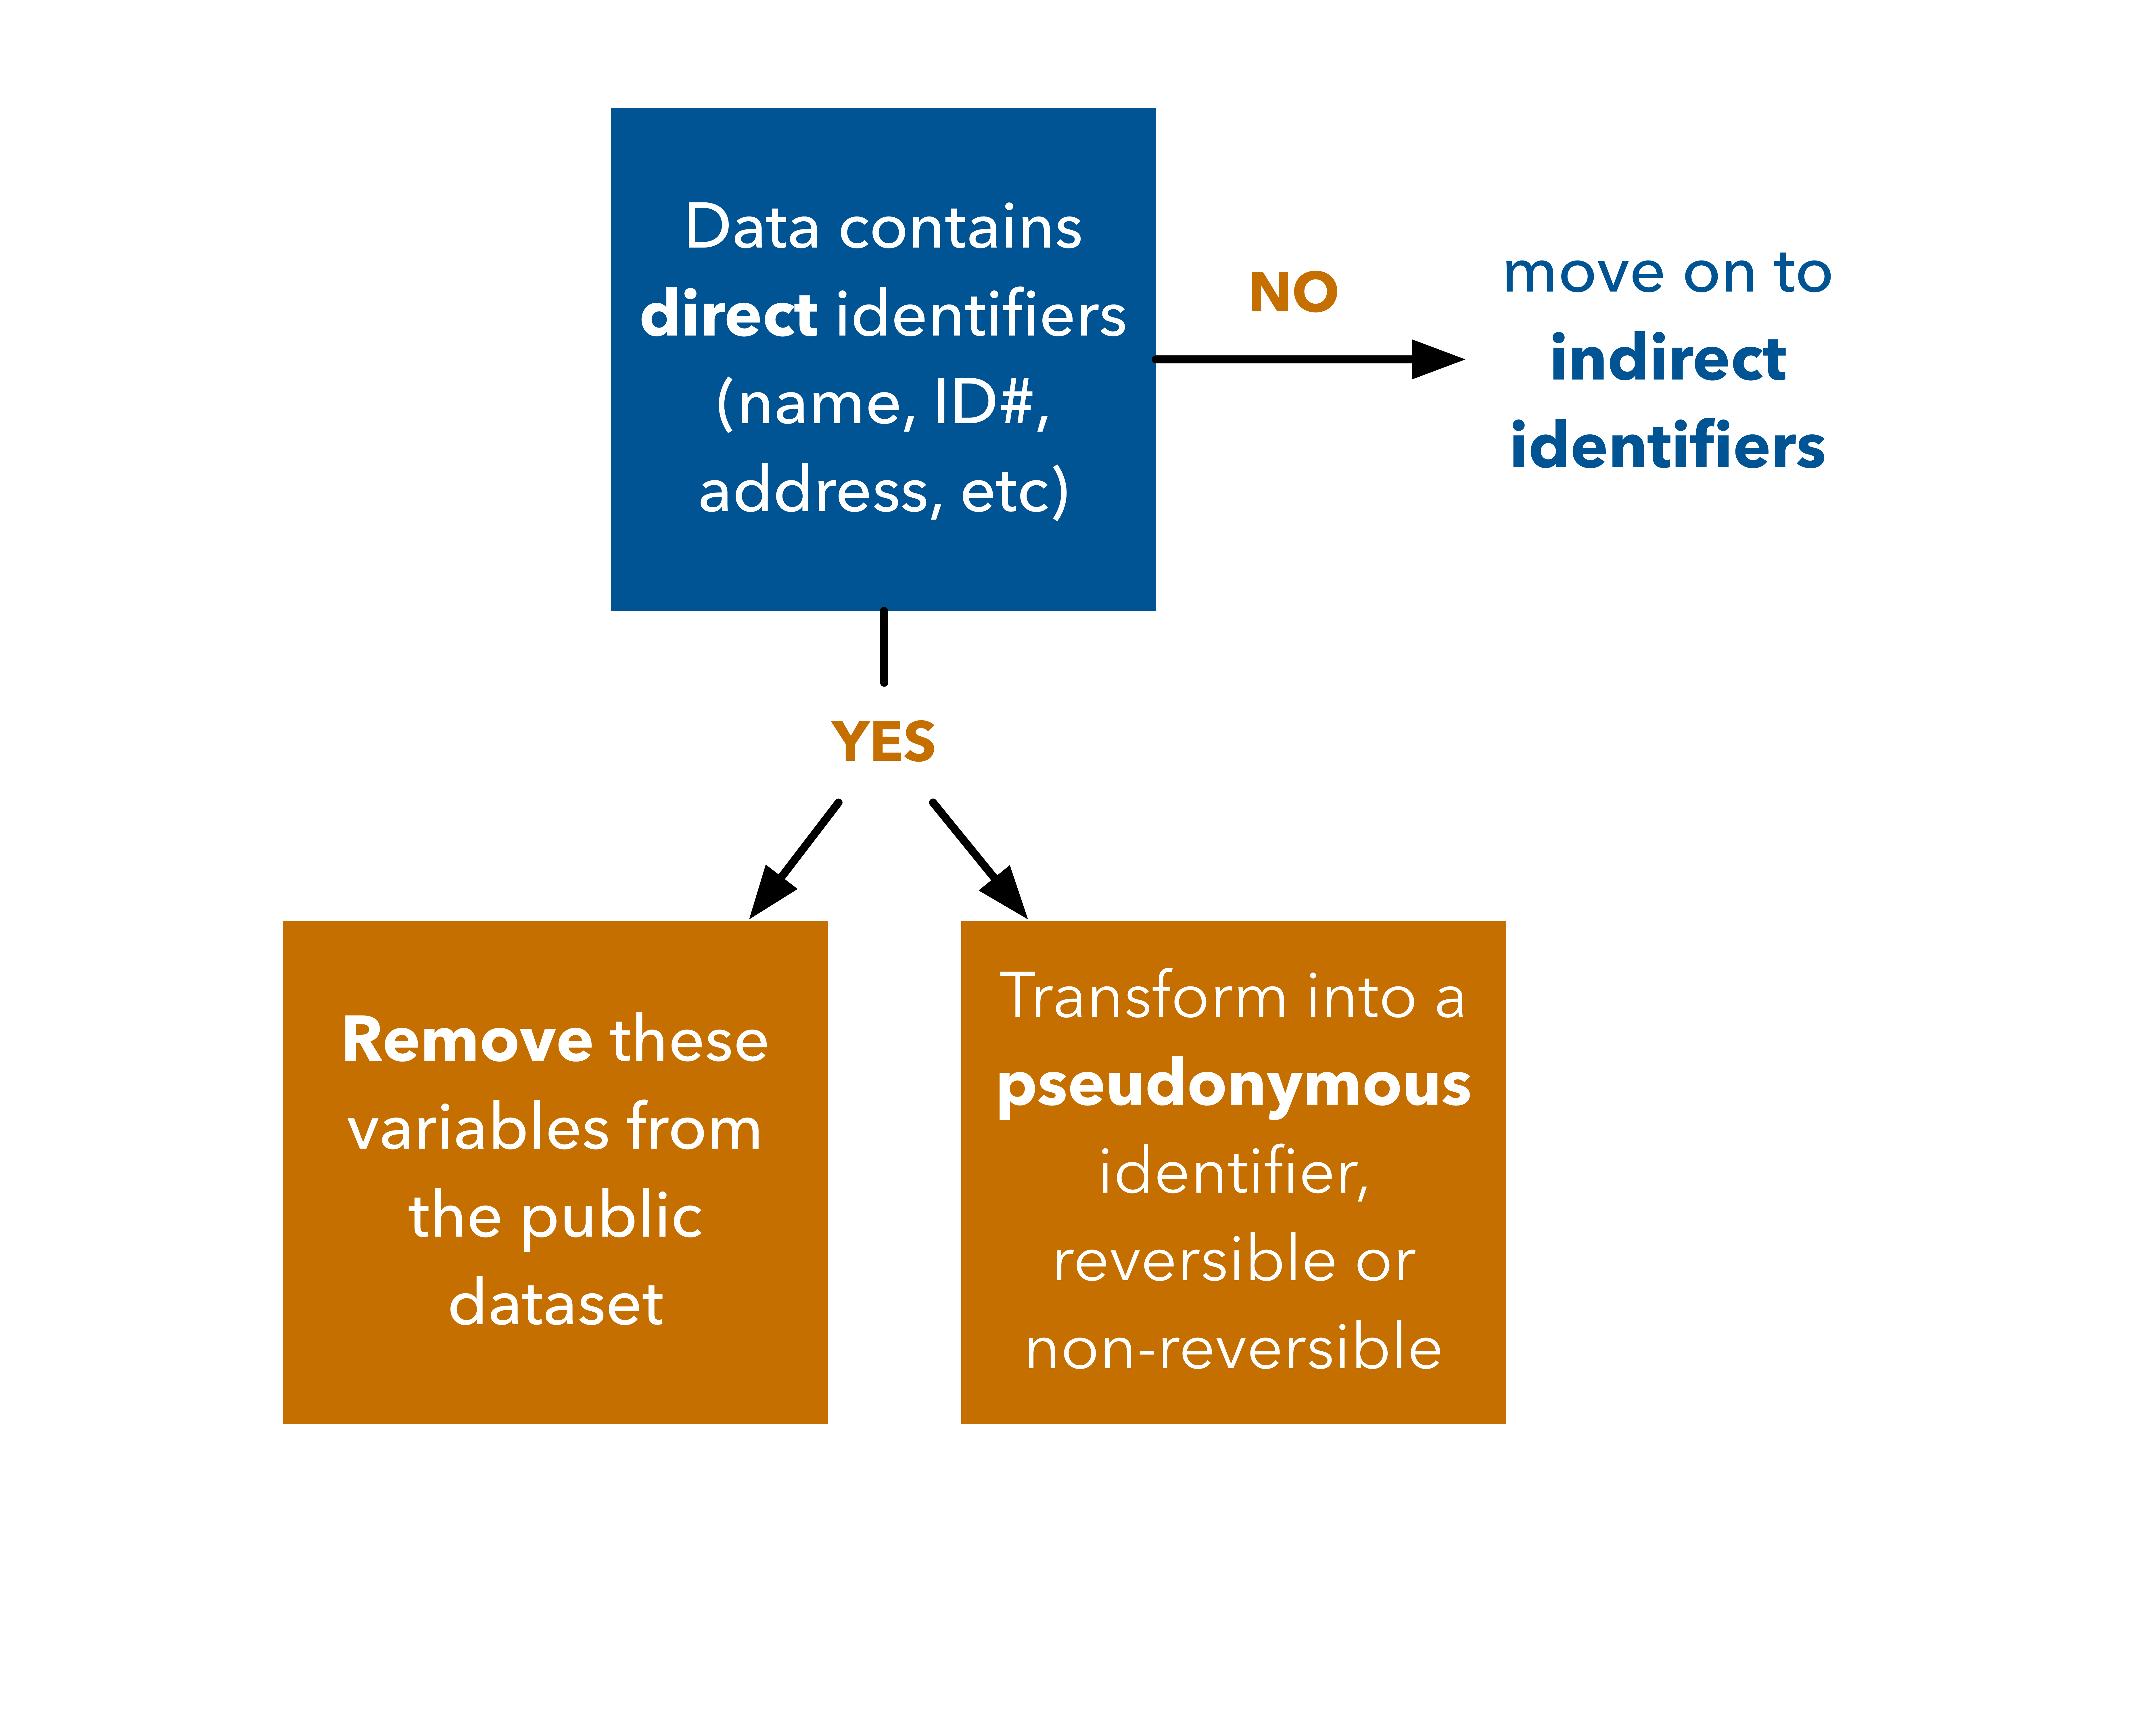
\includegraphics[width=.9\textwidth]{de-identification_direct.png}
	\end{frame}
	
	\begin{frame}{What is sufficient de-identification for indirect identifiers?}
	
		\begin{enumerate}
			\item \textbf{Determine Risk:} Pr(being identified) $\times$ sensitivity of data
			\item \textbf{Set ``k-anonymous" level:} each record cannot be distinguished from at least $k-1$ other individuals who also appear in the data set
			\item \textbf{Select appropriate method(s) of de-identification:} aggregating data, removing certain variables or observations, reducing information/detail, adding random noise or values 
		\end{enumerate}
	\end{frame}
	
	\begin{frame}{Example of K-anon where k=3}
			 \centering 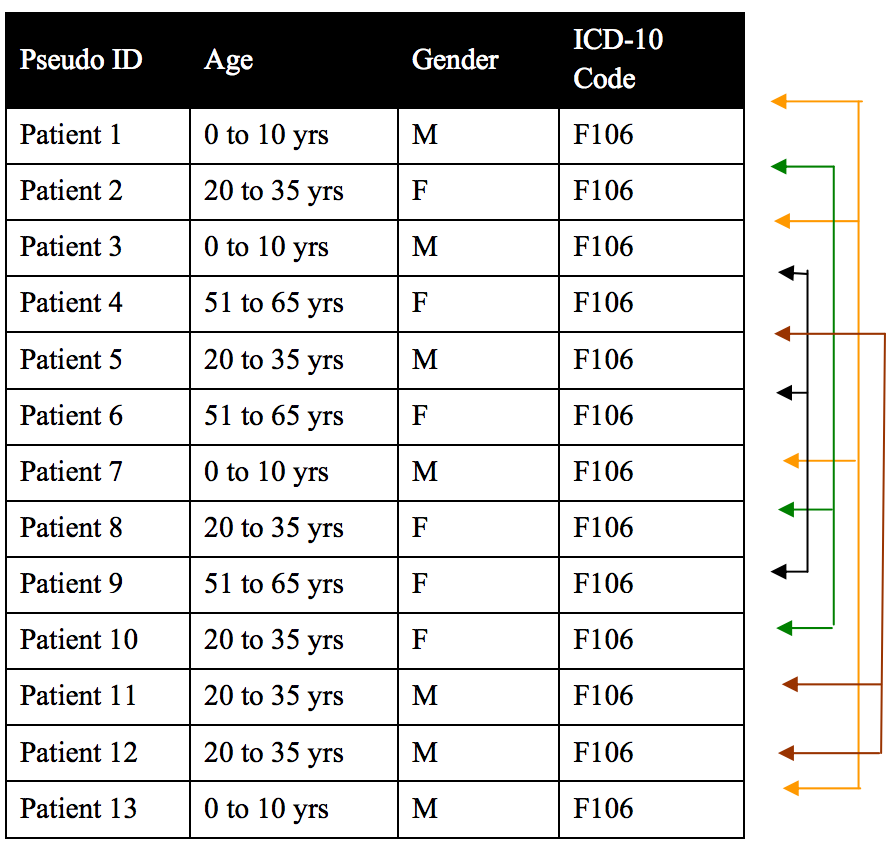
\includegraphics[width=.6\textwidth]{images/k-3.png}
	\end{frame}
	
	\begin{frame}{Solutions for Indirect Identifiers}
		\centering \includegraphics[width=1.1\textwidth]{images/de-identification_indirect.png}
	\end{frame}
	
	\begin{frame}{Trade-off: \textcolor{burntorange}{Usefulness} $\Longleftrightarrow$ \textcolor{burntorange}{Anonymity}}
		
		\pause
		\begin{itemize}
			\item \textbf{Aggregating}---lose ability to replicate any individual-level analysis
			\item \textbf{Removing variables}---may not be able to replicate specific models
			\item \textbf{Remove observations}---adds bias if non-random
			\item \textbf{Reducing information in variables}---adds noise to models
			\item \textbf{Adding random noise/values}---adds noise (obviously)
		\end{itemize}	
	
		\pause
		\bigskip
			See \href{http://www.ehealthinformation.ca/wp-content/uploads/2014/08/2010-Risk-based-de-identification-of-health-data.pdf}{here} and \href{http://www.ehealthinformation.ca/wp-content/uploads/2014/08/2009-Tools-for-De-Identification-of-Personal-Health.pdf}{here} for more discussion of appropriate thresholds, methods, and tools for de-identification.

	\end{frame}
	
	\begin{frame}{Good Practices}
			\begin{itemize}
				\item Include all code even if it manipulates/analyzes identified data, \textit{as long as} it doesn't compromise anonymity---e.g., censor code that sets the seed for a random draw to generate pseudonymous ID numbers
				\item If identifiers \textit{aren't} used for analysis, de-identify early in merging/cleaning process
				\item Store original data with PII securely---if you're using Dropbox, see \href{https://github.com/PolicyDesignEvaluationLab/Transparency-Initiative/wiki/Tips:-Protocol-for-Sharing-Data-via-Dropbox}{PDEL GitHub wiki} for tips on sharing with RAs in a way that protects PII data
			\end{itemize} 	
	\end{frame}
		
 	\begin{frame}{4. Edit and Organize Files for Clarity}
 		Next step is to clean and annotate data, code, and other files to improve usability. 
	 	\bigskip
	 	
	 	\pause
	 	\textbf{Purpose:}
	 		\begin{itemize}
	 			\item Ensure files are \textcolor{burntorange}{legible} in terms of structure and content
	 		\end{itemize}
 	\end{frame}
  
 	\begin{frame}{Basic steps}
 		\begin{itemize}
 			\item Structure and name files*
 			\item Streamline and annotate code*
 			\item Document file and folder contents
 		\end{itemize}
 		
 		\pause
 		\bigskip
 		\nb{*Already done if you follow the literate programming tips in Phase II!}
 	\end{frame}
 
	\begin{frame}{Document File and Folder Content}
		\begin{itemize}
			\item Update the README file to describe contents of replication folders
			\item If necessary, include codebook in ``\texttt{extra/}" folder
			\item Document packages \& software versions used
			\begin{itemize}
				\item \textbf{R:} \texttt{sessionInfo()}
				\item \textbf{Stata:} \texttt{version}
			\end{itemize}
		\end{itemize}
	\end{frame}
	
	\begin{frame}{5. Final Replication}
				
			\begin{itemize}
				\item Shutdown or clear your Stata/R/etc. memory
				\item Rerun the entire process---merging, cleaning and analysis---to make sure your edits didn't break anything
				\item Testing on a friend (or RA's) computer can also be a final check
				\item Once discrepancies are addressed, the files are ready for sharing!
			\end{itemize}
		
	\end{frame}

%%%%% SHARE DATA AND CODE	
		
\subsection{7. Share Data and Code}

	\begin{frame}{About Sharing Data and Code}
		\begin{itemize}
			\item \textbf{What:} add replication files to an \nb{online repository}
			\item \textbf{Why:} lasts longer than personal website, more searchable, future proof
			\item \textbf{Concerns:} 
				\begin{itemize}
					\item Can usually be embargoed, or provide only what is necessary for replication (e.g., unused survey Qs)
					\item Biggest risk isn't having your data/ideas stolen, it's having your research ignored! (King 1995)
					\item Difficult if proprietary
				\end{itemize}
		\end{itemize}
	\end{frame}
	
	\begin{frame}{Where to Share}
		Depends on discipline: find appropriate registry at \url{http://www.re3data.org/}, or check out ... 
		\pause
		\begin{itemize}
			\item \textbf{\href{https://dataverse.harvard.edu/}{Harvard’s Dataverse} }
			\item \href{https://osf.io/}{Open Science Framework}
			\item \href{https://www.openicpsr.org/openicpsr/}{OpenICPSR}
			\item \href{https://figshare.com/}{figshare}
			\item \href{http://datadryad.org/}{Data Dryad}
			\item University library (e.g., \url{http://library.ucsd.edu/dc/rdcp/collections})
		\end{itemize}		
	\end{frame}

%%%%% META-ANALYSIS	

\subsection{8. Meta-Analysis}
	
	\begin{frame}{About Meta-Analysis}
		\begin{itemize}
			\item \textbf{What:} Statistical analysis of a group of studies to derive a pooled estimate of the effect of a treatment; may be part of a ``systematic review" 
			\item \textbf{Why:} Because any estimate in an individual study may be biased or contain random error (note: assumes NO publication bias!)
		\end{itemize}
	\end{frame}

	\begin{frame}{One Study = One Data Point}
		That experiment you just ran with 3,685 participants? It's one data point among many other potential studies. 
		
		\begin{itemize}
			\item What if the results are due to random chance?
			\item What if there was bias in your sample?
			\item What if someone else had analyzed your data?
		\end{itemize}
	\end{frame}
	
		
	\begin{frame}{Even with the same data, results may vary ...}		
		\centering
		\ig[width= \textwidth]{truth-vigilantes-soccer-calls2}
		
		\small \textit{Source:} Graph = fivethirtyeight.com, see \url{https://osf.io/j5v8f/} for study materials
	\end{frame}
	
	\begin{frame}{Basic Steps}
	Using a PAP or ``protocol" ...
	
		\pause
		\begin{enumerate}
			\item Determine which studies to include 
			\item Determine which outcomes to measure (e.g., discrete, continuous)
			\item Select model for ``meta-regression" (e.g., RE, FE, etc.)
		\end{enumerate}
	\end{frame}
	
	\begin{frame}{Funnel Plots}
		Scatter plot of study effect sizes vs. precision (e.g., SE of treatment effect)
		
		\bigskip \centering
		\ig[width=.8\textwidth]{funnel.png}	
		
		\small \textit{Source: BMJ 2011}
	\end{frame}
	
		\begin{frame}{Who does meta-analysis?}
		\begin{itemize}
			\item \href{https://www.campbellcollaboration.org/}{Campbell Collaboration} (policy)
			\item Cochrane Collaboration (medicine)
			\item \href{http://www.3ieimpact.org/}{3ie} (development)
			\item What Works Clearinghouse (US Gov’t, Education) 
			\item CLEAR (US Gov’t, Labor)
			\item MAER-NET (Economics)
			\item You!
		\end{itemize}
	\end{frame}
	
%%%%%%%%%%%%%% ETC. %%%%%%%%%%%%%%%%%
\section{Extra}
\subsection{}

\begin{frame}{Solutions at the Institutional/Discipline Level}
	\begin{itemize}
		\item \textbf{Design-based publication:} AKA ``registered reports," moves peer review before data analysis (\href{https://osf.io/8mpji/wiki/home/}{example})
		\item \textbf{Incentives for transparency, replication, meta-analysis:} See BITSS \href{http://www.bitss.org/lr-prizes/}{prizes} and \href{http://www.bitss.org/ssmart-grants/}{awards}, \href{https://osf.io/prereg/}{OSF pre-registration challenge}, etc.
		\item \textbf{Change norms:} e.g., journal/disciplinary standards for data sharing
		\item \textbf{Training:} Like this! More at BITSS, \href{https://cos.io/our-services/training-services/}{Center for Open Science}, etc.  
		\item \textbf{Tenure:} ``Adherence to the replication standard should be part of [tenure] judgment" (King 1995)
	\end{itemize}
\end{frame}

\begin{frame}{Selected Reading}
\footnotesize
\begin{itemize}
	\item \textbf{Transparency:} \href{https://github.com/garretchristensen/BestPracticesManual}{BITSS Best Practices Manual}
	\item \textbf{Replication:}  \href{http://www.jstor.org/stable/1806061?seq=1\#fndtn-page\_scan\_tab\_contents}{Dewald et al. (1986)}, \href{http://gking.harvard.edu/files/replication.pdf}{King (1995)}, \href{http://www.pnas.org/content/109/42/17028.long}{Fang et al. (2012)}, \href{https://fivethirtyeight.com/features/science-isnt-broken/}{FiveThirtyEight (2015)}, \href{https://www.cgdev.org/sites/default/files/CGD-Working-Paper-399-Clemens-Meaning-Failed-Replications.pdf}{Clemens (2015)}
	\item \textbf{Publication bias:} \href{http://www.nejm.org/doi/full/10.1056/nejmsa065779}{Turner et al. (2008)}, \href{http://journals.sagepub.com/doi/pdf/10.1177/0049124108318973}{Gerber \& Malhotra (2008)} \href{http://journals.plos.org/plosone/article?id=10.1371/journal.pone.0010068}{Fanelli (2010)}, \href{https://link.springer.com/article/10.1007/s11192-011-0494-7}{Fanelli (2011)}, \href{http://science.sciencemag.org/content/345/6203/1502}{Franco et al. (2014)}
	\item \textbf{P-hacking, fishing, researcher degrees of freedom, fraud:} \href{https://papers.ssrn.com/sol3/papers.cfm?abstract_id=1850704}{Simons, Nelson, Simonsohn (2011)}, \href{http://www.stat.columbia.edu/~gelman/research/unpublished/p_hacking.pdf}{Gelmen \& Loken (2013)}, \href{https://www.aeaweb.org/articles?id=10.1257/app.20150044}{Brodeur et al. (2016)}, \href{https://www.cmu.edu/dietrich/sds/docs/loewenstein/MeasPrevalQuestTruthTelling.pdf}{John et al. (2012)}
	\item \textbf{PAPs:} \href{https://www.aeaweb.org/articles?id=10.1257/jep.29.3.61}{Olken 2013}, \href{https://www.aeaweb.org/articles?id=10.1257/jep.29.3.81}{Coffman \& Niederle (2015)}, \href{http://onlinelibrary.wiley.com/doi/10.1111/0019-8676.00199/full}{Neumark 2001}
	\item \textbf{De-identifying data:} \href{http://www.ehealthinformation.ca/wp-content/uploads/2014/08/2009-Tools-for-De-Identification-of-Personal-Health.pdf}{Tools for De-Identification}, \href{http://www.ehealthinformation.ca/wp-content/uploads/2014/08/2010-Risk-based-de-identification-of-health-data.pdf}{El Emam (2010)}
	\item \textbf{Literate programming:} \href{https://www.amazon.com/Workflow-Data-Analysis-Using-Stata/dp/1597180475}{Long (2008)}, \href{https://www.amazon.com/Reproducible-Research-Studio-Chapman-Hall/dp/1466572841}{Gandrud (2013)}, \href{http://www.brown.edu/Research/Shapiro/pdfs/CodeAndData.pdf}{Gentzkow \& Shapiro (2014)}
	\item \textbf{Meta-analysis:} \href{http://www.jstor.org/stable/2117925?seq=1\#page\_scan\_tab\_contents}{Card \& Krueger (1995)}, \href{https://www.amazon.com/Meta-Regression-Analysis-Economics-Business-Routledge/dp/0415670780}{Stanlet \& Doucouliagos (2012)}, \href{http://www.bmj.com/content/343/bmj.d4002}{BMJ (2011)}
	\end{itemize}

\end{frame}

\begin{frame}{}
	\large \centering
	\nb{Thank you!}
\end{frame}

\begin{frame}{About this Presentation}
	\footnotesize
	This presentation was developed by Julia Clark, Scott Desposato, and Craig McIntosh of UCSD's Policy Design and Evaluation Lab (\href{https://pdel.ucsd.edu/}{PDEL}) as part of an effort to integrate good research transparency practices into methods training at UCSD.
	 
	\bigskip
	Funding for this project was generously provided by the Berkeley Initiative for Transparency in the Social Sciences (\href{http://www.bitss.org/}{BITSS}) through a \href{http://www.bitss.org/catalysts}{Catalyst grant}. 
	
	\bigskip
	This presentation and associated materials are available online at \href{https://github.com/PolicyDesignEvaluationLab/Transparency-Initiative}{GitHub} and are licensed under CC BY-NC 4.0 \ig[width = 15mm]{cc_license.png}. You are free to share and adapt them for any non-commercial purpose with proper attribution. Please cite as ``Clark, J., Desposato, S., and McIntosh, C. 2017. `How to improve the credibility of (your) social science: A practical guide for researchers'. Policy Design and Evaluation Lab (PDEL). University of California, San Diego." 
	\end{frame}


\end{document}